\documentclass[12pt, a4paper, portrait]{article}
\usepackage[margin = 2cm]{geometry}
% Vertical text spacing
\parindent = 0cm \parskip = 0cm
% Section
\usepackage[compact]{titlesec} \titlespacing*{\section}{0pt}{2ex}{2ex}
\titleformat*{\section}{\normalfont\Large\bfseries\color[RGB]{0,0,192}}
% Table spacing
\newcommand\TS{\rule{0pt}{2.6ex}}         % Top strut
\newcommand\BS{\rule[-0.9ex]{0pt}{0pt}}   % Bottom strut
\usepackage{array}
\newcolumntype{L}[1]{>{\raggedright\TS\BS\arraybackslash}m{#1}}   % Align left
\newcolumntype{C}[1]{>{\centering  \TS\BS\arraybackslash}m{#1}}
\newcolumntype{R}[1]{>{\raggedleft \TS\BS\arraybackslash}m{#1}}   % Align right
% Equations
\usepackage{amsmath, bm, bbold, pgfplots}

\begin{document}
Dongxiao Huang, Zheng Xun Phang, Yufeng Zhang
\section*{Implementation}
We select the best attribute at each node by computing its information gain, which is the decrease in entropy of the dataset after it has been split on that attribute.
\begin{align*}
    \text{Gain(Attribute)} &= I(p, n) - \left[ \frac{p_0 + n_0}{p + n} \, I(p_0, n_0) + \frac{p_1 + n_1}{p + n} \, I(p_1, n_1) \right] \\[0.5ex]
    p &= \text{Number of positive examples before split} \\
    n &= \text{Number of negative examples before split} \\
    p_k &= \text{Number of positive examples with attribute} = k \\
    n_k &= \text{Number of negative examples with attribute} = k \\
    I(p, n) &= - \frac{p}{p+n} \log \frac{p}{p+n} - \frac{n}{p+n} \log \frac{n}{p+n}
\end{align*}
We could have used another information metric such as the Gini impurity:
\[ I(p, n) = \frac{p}{p+n} \left( 1 - \frac{p}{p+n} \right) + \frac{n}{p+n} \left( 1 - \frac{n}{p+n} \right) \]
which should give similar results to entropy since their graphs have a similar shape:
\begin{center}
\begin{minipage} {0.45 \textwidth}
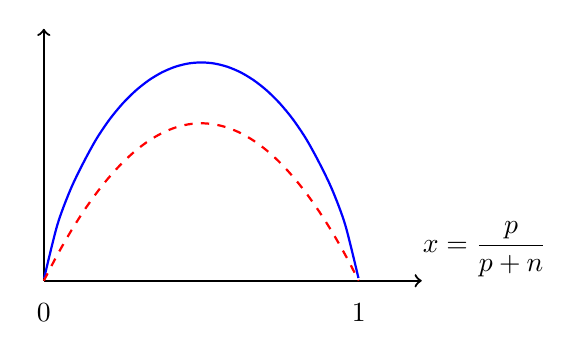
\begin{tikzpicture} [xscale = 4, yscale = 4]
    \draw[->, thick] (0, 0) -- (1.2, 0); 
    \node at (1.4, 0.1) {$\displaystyle x = \frac{p}{p+n}$};
    \draw[->, thick] (0, 0) -- (0, 0.8);
    \newcommand{\gini}[2]    {plot[smooth, domain = #1:#2] (\x, {2 * \x * (1-\x)}) };
    \newcommand{\entropy}[2] {plot[smooth, domain = #1:#2] (\x, {-\x * ln(\x) - (1-\x) * ln(1-\x)}) };
    \draw[thick, blue] \entropy{0.001}{0.999};
    \draw[dashed, thick, red] \gini{0}{1};
    \node at (0, -0.1) {0};
    \node at (1, -0.1) {1};
\end{tikzpicture}
\end{minipage}
\begin{minipage} [b] {0.4 \textwidth}
    {\color{blue} Entropy: $-x \log x - (1-x) \log (1-x)$} \\
    \\
    {\color{red} Gini: $2x (1-x)$}
\end{minipage}
\end{center}

To evaluate our decision tree, we performed cross validation as follows:
\begin{enumerate}
    \item Shuffle the dataset and split it into $K = 10$ parts
    \item For each $k \in \{1, \dotsm, K\}$ we train the decision tree on the dataset \textbf{excluding} part $k$ and then test the decision tree on part $k$.
\end{enumerate}

\section*{Evaluation}
Confusion matrix:
\begin{center}
\begin{tabular} { C{1.7cm} | C{1.5cm} C{1.5cm} C{1.3cm} C{1.7cm} C{1.5cm} C{1.5cm} }
    & Anger & Disgust & Fear & Happiness & Sadness & Surprise \\ \hline
    Anger     &   &   &   &   &   &   \\
    Disgust   &   &   &   &   &   &   \\
    Fear      &   &   &   &   &   &   \\
    Happiness &   &   &   &   &   &   \\
    Sadness   &   &   &   &   &   &   \\
    Surprise  &   &   &   &   &   &
\end{tabular}
\end{center}
Precision\par
Recall\par
$F_1$ score\par

\section*{Miscellaneous}

\textit{Noisy-Clean Datasets Question}\par
\bigskip
The noisy dataset has lower performance.\par
\bigskip

\textit{Ambiguity Question}\par
\bigskip

\textit{Pruning Question}\par
\bigskip

\end{document}
